%\documentclass{article}
%\usepackage{graphicx,subfigure}
%\begin{document}

\begin{figure}[!h]
  \centering
  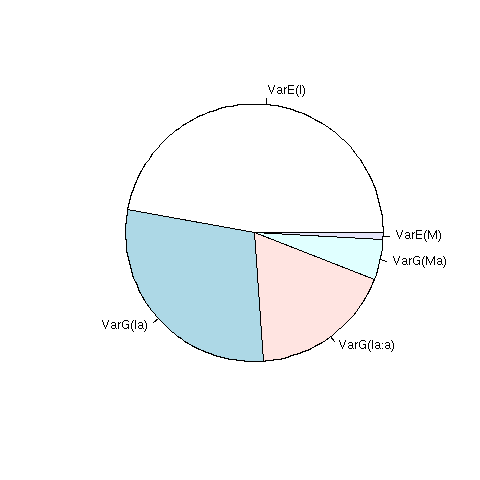
\includegraphics[width=1.0\textwidth]{qgwrinpie.png}
  \caption{Summary of analyses of quantitative genetic variation in wrinkle score. The piechart shows percentages of variation attributed to the following variance components: VarE(I) = individual environmental variance, VarG(Ia) = individual additive genetic variance, VarG(Ia:a) = individual additive x additive epistatic variance, VarG(Ma) = maternal additive genetic variance, and VarE(m) - maternal environmental variance. The variance components are averages of estimates for five Merino flocks.}
  \label{fig:qgwrin}
\end{figure}

%\end{document}

